\documentclass[11pt]{elsarticle}


\usepackage{amsmath}
\usepackage{amsthm}
\usepackage{fullpage}
\usepackage{stmaryrd}
\usepackage{amsfonts}
\usepackage{amssymb}
\usepackage{float}
\usepackage{url}
\usepackage{hyperref}
\usepackage{tikz}
  \usetikzlibrary{automata}
  \usetikzlibrary{arrows}
  \usetikzlibrary{shapes}
  \usetikzlibrary{decorations.pathmorphing}
  \usetikzlibrary{fit}
  \usetikzlibrary{matrix}
  \tikzstyle{every picture}=[
    >=stealth', shorten >=1pt, node distance=1.44cm,auto,bend angle=45,initial text=,
    every state/.style={inner sep=0.75mm, minimum size=1mm},font=\scriptsize,
  ]
\usepackage{algorithm}
\usepackage{algorithmic}

\newsavebox\dotbox
\sbox{\dotbox}{}
\DeclareMathOperator*{\bigcdot}{\raisebox{0pt}[\ht\dotbox][\dp\dotbox]{}}
\newcommand*{\DashedArrow}[1][]{\mathbin{\tikz [baseline=-0.25ex,-latex, dashed,#1] \draw [#1] (0pt,0.5ex) -- (1.3em,0.5ex);}}\newcommand*{\Arrow}[1][]{\mathbin{\tikz [baseline=-0.25ex,-latex, #1] \draw [#1] (0pt,0.5ex) -- (1.3em,0.5ex);}}

\newcommand{\Intervalle}[2]{\{#1,\ldots,#2\}}
\newcommand{\cqfd}{\hfill{\vrule height 3pt width 5pt depth 2pt}}
\newcommand{\Card}[1]{\mathrm{Card}(#1)}
\newcommand{\indef}{\bot}

\newtheorem{definition}{Definition}
\newtheorem{theorem}{Theorem}
\newtheorem{lemma}{Lemma}
\newtheorem{proposition}{Proposition}
\newtheorem{corollary}{Corollary}
\newdefinition{example}{Example}
\newdefinition{question}{Question}

\bibliographystyle{elsarticle-num} 







\usepackage{etoolbox}
\newcommand\modif[2]{{#2}}
  

\begin{document} 

\begin{frontmatter}

  \title{(k,l)-Unambiguity and Quasi-Deterministic Structures}
  
  \author[rouen]{Pascal Caron}
     \ead{pascal.caron@univ-rouen.fr}
  \author[lehavre]{Marianne Flouret}
    \ead{marianne.flouret@univ-lehavre.fr}
  \author[depart]{Ludovic Mignot} 
     \ead{ludovic.mignot@univ-rouen.fr}
  

  \address[rouen]{LITIS, Universit\'e de Rouen, 76801 Saint-\'Etienne du Rouvray Cedex, France}

  \address[lehavre]{LITIS, Universit\'e du Havre, 76058 Le Havre Cedex, France}
    \address[depart]{D\'epartement d'informatique, Universit\'e de Rouen, 76801 Saint-\'Etienne du Rouvray Cedex, France}

  \begin{abstract} 
We focus on the family of -unambi\-guous automata that encompasses the one of deterministic -lookahead automata introduced by Han and Wood.
    We show that this family presents nice theoretical properties that allow us to compute quasi-deterministic structures. 
    These structures are smaller than DFAs and can be used to solve the membership problem faster than NFAs.    
  \end{abstract}
  
	\begin{keyword}
	  Automata theory \sep Deterministic automata \sep -lookahead determinism \sep Unambiguity 
	  \MSC[2010] 68Q45  
	\end{keyword}
\end{frontmatter}



\section{Introduction}\label{se:int}
  \modif{This paper is an extended version of~\cite{CFM14}.}{}

One of the \modif{best known}{most popular} automata construction is the position automaton construction \cite{Glu61}. If a regular expression has  occurrences of symbols, then the corresponding position automaton, which is not necessarily deterministic, has exactly  states.
  The -unambiguous  regular languages have been defined by Br\"uggemann-Klein and Wood~\cite{BW98} as  languages denoted  by  regular expressions  the position automata of which are deterministic. They have also shown that there exist regular languages that are not -unambiguous. This property has practical implication, since it models a property needed in XML DTDs~\cite{BPS06}. Indeed, XML DTDs are defined as an extension of classical context-free grammars in which the right hand side of any production is a one-unambiguous regular expression. 
   Consequently, \modif{}{a} characterization of such languages, \modif{that}{which} has been considered \emph{via} the deterministic minimal automaton, is very important, since it proves that not all the regular languages can be used in XML DTDs.  
  The computation of a small deterministic recognizer is also technically important since it allows a reduction of the time and of the space needed to solve the membership problem (to determine whether or not a given word belongs to a language).
   As a consequence, one may wonder whether there exists a family of languages encompassing the -unambiguous one that can be recognized by a polynomial-size deterministic family of recognizers.


  On the one hand, numerous extensions of -unambiguity have been considered, like -block determinism~\cite{GMW01}, -lookahead determinism~\cite{HW08} or weak -unambiguity~\cite{CHM11}. All of these extensions, likely to the notion of -unambiguity, are expression-based properties. A regular language is -unambiguous (resp. -block deterministic, -lookahead deterministic, weakly -unambi\-guous) if it is denoted by a -unambiguous (resp. -block deterministic, -lookahead deterministic, weakly -unambi\-guous) regular expression. All of these three properties are defined through a recognizer construction.
  
  On the other hand, the concept of lookahead delegation, introduced in \cite{DIS04}, handles determinism without computing a deterministic recognizer; the determinism is simulated by a fixed number of input symbols read ahead, in order to select the \emph{right} transition in the NFA. This concept arose in a formal study of web-services composition and its practical applications~\cite{GHIS04}. Questions about complexity and decidability of lookahead delegation have been answered by Ravikumar and Santean in~\cite{RS07}. Finally, having defined predictable semiautomata, Brzozowski and Santean~\cite{BS09} improved complexity of determining whether an automaton admits a lookahead delegator.
  
  The notion of -unambiguity for automata is the first step of the study of the -unambiguity for languages. In this paper,  
   we define the notion of -unambiguity for automata, leading to the computation of quasi-deterministic structures, that are smaller than DFAs and that can be used to solve the membership problem faster than NFAs.    
  These structures act as automata for which a window of size  and some shifting states are added. Recognizing a word on such a structure is performed as follows: At the beginning of the process, the window matches the  first letters of the input word. When a shifting state is reached and the input word is not entirely read, the window is slided along the input word ( letters, depending on the shifting state), the \modif{QDS}{Quasi-Deterministic Structures (QDS)} returns in a regular state and the reading restarts at the beginning of the window.
  We then show, thanks to an equivalence relation, how to reduce such structures. We also exhibit a family of languages for which reduced QDS are exponentially smaller than minimal DFAs.
  Next step is to study the -unambiguous languages, that are languages denoted by some  regular expressions the position automaton of which is -unambiguous. Having such a regular expression allows us to directly compute a quasi-deterministic structure to solve the membership problem.
  
  In Section~\ref{se:klna}, after defining the -unambiguity as an extension of -lookahead determinism, we characterize this notion making use of the \emph{square automaton}. 
  In Section~\ref{se:qds}, we define quasi-deterministic structures that allow us to perform a constant space membership test. Section~\ref{se:klnanfa2qds} is devoted to the computation of the quasi-deterministic structure associated with a -unambiguous automaton. The notion of quotient of a quasi-deterministic structure is defined in Section~\ref{sec qds}, and a right invariant equivalence relation is investigated. It is shown in Section~\ref{sec qds vs dfa} that reduced quasi-deterministic structures can be exponentially smaller than minimal \modif{deteministic}{deterministic} automata.
  
  \modif{}{This paper is an extended version of~\cite{CFM14}.}

\section{Preliminaries}\label{se:pre}

Let  be \emph{the empty word}. An \emph{alphabet}  is a finite set of distinct symbols. The usual concatenation of symbols is denoted by , and  is its identity element. We denote by  the smallest set containing  and closed under  the  operation. Any subset of  is called a \emph{language over} . Any element of  is called a \emph{word}. The length of a word , noted , is the number of symbols in  \modif{it is the concatenation of}{occurring in }  (\emph{e.g.} ). By extension the number of elements of a set  is denoted by .
For a given integer , we denote by  the set of words of length  and by  the set . 
 Let  be a word in  such that for any  in ,  is a symbol in . 
Let  and  be two integers such that . We denote by  the subword  of  starting at position  and ending at the position  and by  the -th symbol  of .
More generally, we will define by  the word .  In case , this word is .


A \emph{nondeterministic finite automaton} (\textbf{NFA})  is a -tuple  where  is an alphabet,  is a \emph{set of states},  is a \emph{set of initial states},  is a \emph{set of final states} and  is a \emph{transition function} defined from  to . The function  can be interpreted as a subset of  defined by   .
 The domain of  is extended to  as follows: for any symbol  in , for any state  in , for any subset  of , for any word  in : , , . 
  Let   be an integer and  be a word in . A \emph{path}  \emph{labelled by}  is a finite sequence \modif{}{ of states} such that for any integer , . The path  \emph{starts} with . Two paths  and  labelled by  are \emph{totally distinct} if for any integer , .
  A path  is a cycle if  and .  
The automaton  is  \emph{deterministic} if the two following properties hold:  and .
A state  in  is  \emph{accessible} (resp. \emph{coaccessible}) if there exists a word  in  such that  (resp. ). The automaton  is \emph{accessible} (resp. \emph{coaccessible})  if any state in  is accessible (resp. coaccessible). The automaton is \emph{trim} if any state in  is accessible and coaccessible.


Given a word  and an -state automaton , the membership test~\cite{HMU07}, \emph{i.e.} deciding whether  belongs to , can be performed in time  and in space . Let us suppose that  is the  -state deterministic automaton of  (computed as the classical accessible part of the powerset automaton of ). The membership test can be performed in time  and in space , but  can be exponentially greater than .

Glushkov~\cite{Glu61} and McNaughton and Yamada~\cite{MY60} have independently defined the construction of the \emph{Glushkov automaton} or \emph{position automaton}  of a 
regular expression . The number of states  of  is a linear function of the width \modif{}{} of  (\emph{i.e.} the number of occurrences of the symbols of  in ); in fact, \modif{}{}.
The automaton  is a 
-state  automaton that recognizes .

A regular expression  is \emph{deterministic} if and only if its Glushkov automaton is. A language is  -\emph{unambiguous} if there exists a deterministic expression to denote it. Br\"uggemann-Klein and Wood~\cite{BW98} have shown that determining whether a regular language is -unambiguous or not is a decidable problem. Furthermore, they proposed a characterization and showed that both -unambiguous languages and non -unambiguous regular languages exist.

The notion of -lookahead determinism~\cite{HW08} extends the one of -unambi\-guity of expressions. In that purpose, Han and Wood define the \emph{-lookahead deterministic position automaton} of an expression.

\begin{definition}[\cite{HW08}]\label{def kla}
  Let  be a position automaton of an expression. Then  is a \emph{deterministic} \emph{-lookahead automaton} if for any state  in , where , , ,  are the out-transitions of , with  for , it holds: , where  and  is the set of words of length  that labels a path starting at .
\end{definition}

Notice that this definition can be extended to any automaton that is not a position one.
Informally, an automaton is -lookahead deterministic if and only if for any state , for any word  of length , all  paths from  labelled by  have a common first transition  (see Figure~\ref{fig ex general klh}).
\modif{}{An automaton is lookahead-deterministic if there exists an integer  such that it is -lookahead-deterministic.}

\begin{figure}[H]
  \begin{minipage}{0.49\linewidth}
    \centerline{ 
      \begin{tikzpicture}[node distance=1.5cm,bend angle=30]   
	    \node[state] (q) {};
	    \node (q') [right of=q]{};
	    \node[state] (q1) [above right of=q']{};
	    \node[state] (q2) [right of=q']{};
	    \node[state] (q3) [below right of=q']{};
	    \path[->,dashed]
	      (q)   edge node {} (q1)
	      (q)   edge node {} (q2)
	      (q)   edge node {} (q3);	            
      \end{tikzpicture}
    }   
    \end{minipage}
    \hfill    
  \begin{minipage}{0.49\linewidth}
    \centerline{  
      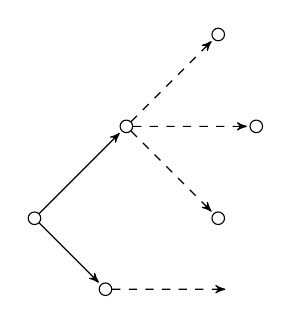
\begin{tikzpicture}[node distance=2.2cm,bend angle=25,transform shape,scale=0.75]   
	    \node[state] (q) {};  
	    \node[state] (q'') [node distance=1.7cm, below right of=q] {};
	    \node (q''') [right of=q''] {};
	    \node[state] (q') [above right of=q]{};
	    \node[state] (q1) [above right of=q']{};
	    \node[state] (q2) [right of=q']{};
	    \node[state] (q3) [below right of=q']{};
	    \path[->]
(q)   edge[swap]  node {} (q'')
	      (q'')   edge[dashed]  node {} (q''')
	      (q)   edge node {} (q')
(q')   edge[dashed] node {} (q1)
	      (q')   edge[dashed] node {} (q2)
	      (q')   edge[dashed] node {} (q3);	            
      \end{tikzpicture}     
    }   
    \end{minipage}
\caption{The -lookahead determinism}
    \label{fig ex general klh}
  \end{figure}
  
  Brzozowski and Santean~\cite{BS09} introduced the notion of predictability for an automaton and linked it to the one of lookahead determinism: as far as an automaton admits a unique initial state, it is -predictable if and only if it is -lookahead deterministic.
  
  In order to decide whether a given automaton is predictable, they make use of the square automaton defined as follows: let . The \emph{square automaton}  of  is the automaton  where for any pair  of states in , for any symbol  in , .
  
  Finally, \modif{from the square automaton,}{} they define the pair automaton\modif{of}{, the subautomaton of the square automaton restricted to the} critical subsets of  (the set of initial states and the sets of successors of a \modif{fork}{state with at least two distinct successors}). An automaton is predictable if and only if its pair automaton admit no cycle. A closely related method has already been applied in comparable settings for Moore machines~\cite{Koh90}.

\section{The (k,l)-unambiguity}\label{se:klna}



  The definition of -lookahead determinism can be extended by the introduction of an additional parameter . The maximal length of ambiguity in two distinct paths from the same state and labelled by a same word is bounded by this parameter. Hence\modif{}{,} an automaton is said to be -unambiguous () if and only if for any state , for any word  of length , if there exist at least two distinct paths from  labelled  by ,  then there exists an integer  such that all these paths share a common successor after a path of length  (see Figure~\ref{fig ex general klna}).

 
\begin{figure}[H]
  \begin{minipage}{0.49\linewidth}
    \centerline{ 
      \begin{tikzpicture}[node distance=1.5cm,bend angle=30]   
	    \node[state] (q) {};
	    \node (q') [right of=q]{};
	    \node[state] (q1) [above right of=q']{};
	    \node[state] (q2) [right of=q']{};
	    \node[state] (q3) [below right of=q']{};
	    \path[->, dashed]
	      (q)   edge node {} (q1)
	      (q)   edge node {} (q2)
	      (q)   edge node {} (q3);	            
      \end{tikzpicture}
    }   
    \end{minipage}
    \hfill    
  \begin{minipage}{0.49\linewidth}
    \centerline{  
      \begin{tikzpicture}[node distance=2.2cm,bend angle=30,scale=0.8]   
	    \node[state] (q) {};  
	    \node[state] (q'') [node distance=1.8cm, below right of=q] {};
	    \node (q''') [node distance=2cm, right of=q''] {};
	    \node[state] (q') [above right of=q]{};
	    \node[state] (q1) [above right of=q']{};
	    \node[state] (q2) [right of=q']{};
	    \node[state] (q3) [below right of=q']{};
	    \path[->,dashed]
	      (q)   edge [bend left] node {} (q')
	      (q)   edge[swap]  node {} (q'')
	      (q'')   edge [swap] node {} (q''')
	      (q)   edge node {} (q')
	      (q)   edge[bend right] node {} (q')
	      (q')   edge node {} (q1)
	      (q')   edge node {} (q2)
	      (q')   edge node {} (q3);	            
      \end{tikzpicture}     
    }   
    \end{minipage}
\caption{The -unambiguity}
    \label{fig ex general klna}
  \end{figure} 
  
\begin{definition}\label{def aut klna}
  Let  and  be two integers such that . A finite automaton  is -\emph{unambiguous} if  and if for any state  in , for any word  in , there exists an integer  such that:
  
  \centerline{
    .
  }
\end{definition}

As a direct consequence of this definition, it holds that any -unambi\-guous automaton is also a -unambiguous automaton whenever .

The following example enlightens the notion of -unambiguity while illustrating the difference between -unambiguity and -lookahead determinism.
  

\begin{example}\label{ex aut klna pour cas concrets}
  Let us consider the automaton  in Figure~\ref{fig ex aut klna pour cas concrets}.
  Let us notice that for , , for all , . 
As a consequence, the automaton is not -unambiguous.
Increasing the length  of the window allows us to avoid this ambiguity. Indeed, for any word  of length , . Hence  is -unambiguous.
  Furthermore,  is also -unambiguous 
but not -unambiguous.
  Finally, let us notice that this automaton is not -lookahead deterministic for any integer  since for any integer  and for any prefix  of ,  and . 
\end{example}

\begin{figure}[H]
  \centerline{ 
    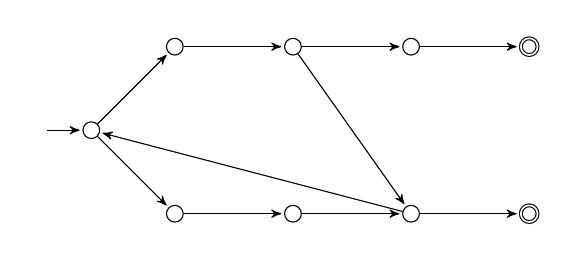
\begin{tikzpicture}[node distance=1.5cm,bend angle=30]   
	    \node[initial,state] (0) {};
	    \node[state] (1) [above right of=0]{};
	    \node[state] (2) [below right of=0]{};
	    \node[state] (3) [right of=1]{};
	    \node[state] (4) [right of=2]{};
	    \node[state] (5) [right of=3]{};
	    \node[state] (6) [right of=4]{};
	    \node[state,accepting] (7) [right of=5]{};
	    \node[state,accepting] (8) [right of=6]{};
	    \path[->]
	      (0)   edge node {} (1)
	      (0)   edge[swap] node {} (2)
	      (1)   edge node {} (3)
	      (2)   edge[swap] node {} (4)
	      (3)   edge node {} (5)
	      (3)   edge node {} (6)
	      (4)   edge[swap] node {} (6)
	      (5)   edge node {} (7)
	      (6)   edge node {} (8)
	      (6)   edge[swap] node {} (0);	            
    \end{tikzpicture}
  }   
  \label{fig ex aut klna pour cas concrets}
  \caption{The automaton of Example~\ref{ex aut klna pour cas concrets}.}
  \end{figure}

\modif{}{Let us now explicit the difference between the -lookahead determinism and the -unambiguity. First, as a direct consequence of Definition~\ref{def kla} and Definition~\ref{def aut klna}, the following proposition holds.}
\begin{proposition}\label{prop eq k1na klh}
  An automaton is deterministic -lookahead if and only if it is  -unambiguous.
\end{proposition}
\modif{\begin{proof}
  Let  be an automaton,  be an integer and  be a state in .
  \begin{enumerate}
    \item Suppose that  is not -unambiguous. Hence there exists a word  of length  such that for any integer :
  
  \centerline{
    .
  }
  
  Then \modif{exists}{exist} two distinct states  and  in  such that    and .
  Either  and  is not deterministic (\emph{i.e.}  is not deterministic -lookahead), or  and by definition of  and , . Hence 
  
  \centerline{
    .
  }
  
  As a consequence,  is not deterministic -lookahead.
  
  \item Suppose that  is not deterministic -lookahead. Then there \modif{exists}{exist} three states ,  and  such that the transitions  and  belongs to  and . Hence there exists a word  of length  such that  and . Consequently the states  and  both belong to the set  and then  is not -unambiguous.
  \end{enumerate}
  
\end{proof}}{}

\begin{proposition}
  \modif{T}{For any integer , t}here exists  a \modif{}{}-unambiguous automaton which is  not \modif{-}{}lookahead deterministic\modif{ for any integer }{}. 
\end{proposition}
\begin{proof}
  An illustration is given in Example~\ref{ex aut klna pour cas concrets}.
  \modif{}{This example can be easily generalized by considering the -unambiguous automaton  in Figure~\ref{general fig ex aut kl}.}
\end{proof}

\modif{}{
\begin{figure}[H]
  \centerline{ 
    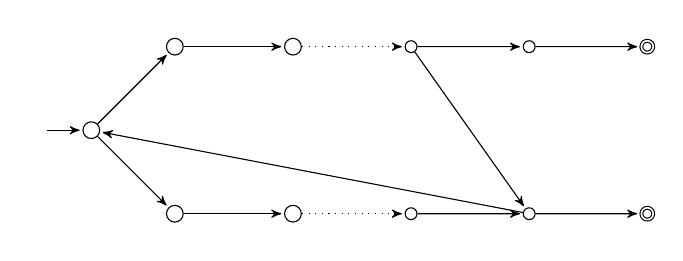
\begin{tikzpicture}[node distance=1.5cm,bend angle=30]   
	    \node[initial,state] (0) {};
	    \node[state] (1) [above right of=0]{};
	    \node[state] (2) [below right of=0]{};
	    \node[state] (2p) [right of=2]{};
	    \node[state] (3) [right of=1]{};
	    \node[state,rounded rectangle] (3p) [right of=3]{};
	    \node[state,rounded rectangle] (4) [right of=2p]{};
	    \node[state,rounded rectangle] (5) [right of=3p]{};
	    \node[state,rounded rectangle] (6) [right of=4]{};
	    \node[state,accepting,rounded rectangle] (7) [right of=5]{};
	    \node[state,accepting,rounded rectangle] (8) [right of=6]{};
	    \path[->]
	      (0)   edge node {} (1)
	      (0)   edge[swap] node {} (2)
	      (1)   edge node {} (3)
	      (2)   edge[swap] node {} (2p)
	      (2p)   edge[swap,dotted] node {} (4)
	      (3)   edge[dotted] node {} (3p)
	      (3p)   edge node {} (5)
	      (3p)   edge node {} (6)
	      (4)   edge[swap] node {} (6)
	      (5)   edge node {} (7)
	      (6)   edge node {} (8)
	      (6)   edge[swap] node {} (0);	            
    \end{tikzpicture}
  }   
  \caption{A -unambiguous automaton.}  \label{general fig ex aut kl}

\end{figure}
}
  


Whenever an automaton is not -unambiguous for any couple  of integers \modif{}{(\emph{e.g.} when two distinct states with a loop can be reached from the same state by the same word)}, there exists a state from which it cannot be decided without ambiguity which successor will appear during the run. Hence there exists an infinite hesitation between two paths, that can be decided \emph{via} the square automaton.

\begin{theorem}\label{theorem caract klna}
  Let  be an accessible automaton and  be the accessible part of its square-automaton. The two following propositions are equivalent:
  \begin{enumerate}
    \item there exists a couple  such that  is -unambiguous,
    \item every cycle in  contains a pair  for some  in .  \end{enumerate}
\end{theorem}

In order to prove Theorem~\ref{theorem caract klna}, let us first state the following lemmas.

\begin{lemma}\label{lem 2chem imp 2 chem tot dis}
  Let  be an automaton,  and . The two following conditions are equivalent:
  \begin{itemize}
\item  for any positive integer , ,
\item  there \modif{exists}{exist} at least two totally distinct paths labelled by  that starts with .
\end{itemize}
\end{lemma}
\begin{proof}
  Let  be an integer. Let  be a word in  and  be a state in  
such that for any integer , . Then there \modif{exists}{exist} two paths  and  labelled by  that starts with . If these two paths are totally distinct, then the lemma is valid, otherwise there exists a third path  such that for any integer ,   . Let us show by recurrence on  that there \modif{exists}{exist} two totally distinct paths  and  from  labelled by  such that . 
  \textbf{(a)} Let us set . Then by definition of , either  or . \modif{R}{The r}ecurrence hypothesis is satisfied.
  \textbf{(b)} Let us set . Let us suppose that there \modif{exists}{exist} two totally distinct paths labelled by . Without loss of generality, let us suppose that  and . If , adding these two distinct states respectively to the paths  and  constructs two totally distinct paths labelled by , otherwise, and without loss of generality, let us suppose that . Since by definition of ,   . Considering  and ,  two totally distinct paths labelled by  are computed.

  
\end{proof}

\modif{}{The  following lemma is straightforward and is useful  for  proving  Theorem~\ref{theorem caract klna}.}

\modif{\begin{lemma}\label{lem 2chem total dis 1 chem car}
  Let  be an automaton and  be its square-automaton. Let  be a word in  and  be a state in . If there \modif{exists}{exist} two totally distinct paths labelled by  that starts with  in , then there exists a path  in  labelled by  starting with  such that for any integer ,  with .
\end{lemma}}{}
\modif{\begin{proof}
  Let  and .
  
  Let  and  be two totally distinct paths labelled by  such that . Let . Let us show by recurrence on the length of  that  is a path in  labelled by  that starts with  such that for any integer ,  with .
  
  Since , it holds that .
  
  Let . Since  and  are two distinct path labelled by , then . Hence, .  Furthermore, since  and  are totally distinct, .
  
  Let . Suppose that for any integer ,  in  is labelled by  starting with  such that for any integer ,  with . Since by definition of  and ,  belongs to  and  belongs to , it holds that  belongs to . Hence . Furthermore, since  and  are totally distinct, .
  
\end{proof}}{}

\begin{lemma}\label{lem q acc ds a qq acc ds car a}
  Let  be an automaton and  be its square-automaton. Let  be a word in  and  and  be two states in . If  then .
\end{lemma}
\modif{\begin{proof}
  By recurrence on the length of .
  
  If , since  and , the recurrence property holds.
  
  Let . Let us suppose that  and . Let . Hence . As a consequence, .
  
\end{proof}}{}

\begin{proof}[\modif{}{Proof of }Theorem~\ref{theorem caract klna}]
Let us set  and .
  
   Let us suppose that there exists a cycle  in  that does not contain any pair  for all state  in . As a consequence, there exists a path  from  to a state  in  such that any predecessor of the first occurrence of  does not belong to . Let  be the state in  such that \textbf{(a)}  appears on the path  from  to the first occurrence of  and \textbf{(b)} there exists no state  in  such that  appears on the path  between  and the first occurrence of . Notice that  exists since  satisfies the previous propositions. Hence for any integer , there exists a word  in  such that  and such that . Consequently, there exists no couple  such that  is -unambiguous.
  
   Let us suppose that for every integer , there exists a word  in  and a state  in  such that 
for any integer , . Hence according to Lemma~\ref{lem 2chem imp 2 chem tot dis}, there \modif{exists}{exist} at least two totally distinct paths labelled by  that start with . Since  is reachable from , then it holds from Lemma~\ref{lem q acc ds a qq acc ds car a} that  belongs to  since it is reachable from . According to the definition of distinct paths, for any integer , there exists a word in  such that there exists a path  in  labelled by  starting with  such that for any integer ,  with . Finally, whenever , there \modif{exists}{exist} two integers  such that . Consequently there exists a cycle in  that contains no pair  for any  in .  
  
  \end{proof}

Notice that Theorem~\ref{theorem caract klna} defines a polynomial decision procedure to test if, for a given NFA , there exists a couple  of integer\modif{}{s} such that  is -unambiguous.

\modif{}{In order to have an upper bound of the complexity of this decision procedure, let us consider a pair automaton   of  states. It is sufficient to remove all the states  of  and to check if the obtained automaton is acyclic, which can be done by applying  times the linear time Tarjan  algorithm \cite{Tar72}  which leads to a complexity in .}

The next section is devoted to the definition of quasi-deterministic structures. These structures allow us to solve the membership problem with the same complexity as deterministic automata 
while being possibly exponentially smaller. Finally, we show in Section~\ref{se:klnanfa2qds} how to convert a -unambiguous NFA into a quasi-deterministic structure.

\section{The quasi-deterministic structure}\label{se:qds}

A quasi-deterministic structure is 
a structure 
derived from an automaton: it embeds a second transition function
 that is 
used to shift the input window 
(of a fixed length) 
while reading a word (see Figure~\ref{fig ex qds graph}). 
In the following, the symbol  is used to represent undefined states and transitions.

\begin{definition}
  A \emph{quasi-deterministic structure} (QDS) is a -tuple   where:
  \begin{itemize}
    \item  is the alphabet of words,
    \item  is the number of levels,
    \item  is the alphabet of shifts,
    \item  is a family of  disjoint set\modif{}{s} of states (levels),
    \item  is the initial state,
    \item  is the set of final states,
    \item  is a \modif{}{total} function from  to  for ,
    \item  is a \modif{}{total} function from  to .  \end{itemize}
  
  The function  can be extended for any state  in ,\modif{ for any state  in ,}{} for any word  in  and for any symbol  in  to , \modif{}{}, , . We will denote  (resp. ) the restriction of the function  to  (resp. ). The functions  and  can also be seen as sets of triplets. An \emph{edge} is an element of . Two edges  and   are consecutive if .
A \emph{path} in a QDS is a sequence   of \modif{}{consecutive} edges.  

\end{definition}



 An example of a QDS is given by Figure \ref{fig ex qds graph}. 
 
\begin{figure}[H]
\begin{minipage}{0.6\linewidth}
\begin{itemize}
\item , , 
\item 
\item 
\item 
\item 
\item 
\end{itemize}
\end{minipage}
\begin{minipage}{0.39\linewidth}
\modif{\begin{tikzpicture}[node distance=2cm,bend angle=30]   
	    \node[initial, state] (1) {};     
	    \node[accepting, state, right of=1] (2) {}; 
	    \node[state, right of=2] (4) {}; 
	    \node[state, above of=2] (3) {};  
	    \node[state, above of=4] (5) {};  
	    \node[state, below of=1] (6) {};  
	    \node[accepting, state, right of=6] (7) {}; 
	    \node[state, right of=7] (8) {};  
	    \path[->]
	      (1)   edge  node {} (2)
	      (1)   edge  node {} (3)
	      (2)   edge  node {} (5)
	      (2)   edge  node {} (4)
	      (3)   edge  node {} (5)
	      (6)   edge  node {} (7)
	      (7)   edge  node {} (8)
	      (5)   edge[dotted,swap, out=135, in = 90]  node {} (1)
	      (4)   edge[dotted]  node {} (6)
	      (8)   edge[dotted,bend left]  node {} (6)
	      ;	            
      \end{tikzpicture}  }{
    \begin{tikzpicture}[node distance=2cm,bend angle=30]   
	    \node[initial, state] (1) {};     
	    \node[accepting, state, right of=1] (2) {}; 
	    \node[state, right of=2] (4) {}; 
	    \node[state, above of=2] (3) {};  
	    \node[state, above of=4] (5) {};  
	    \node[state, below of=1] (6) {};  
	    \node[accepting, state, right of=6] (7) {}; 
	    \node[state, right of=7] (8) {};  
	    \path[->]
	      (1)   edge  node {} (2)
	      (1)   edge  node {} (3)
	      (2)   edge  node {} (5)
	      (2)   edge  node {} (4)
	      (3)   edge  node {} (5)
	      (6)   edge  node {} (7)
	      (7)   edge  node {} (8)
	      (5)   edge[dotted,swap, out=135, in = 90]  node {} (1)
	      (4)   edge[dotted]  node {} (6)
	      (8)   edge[dotted,bend left]  node {} (6)
	      ;	            
      \end{tikzpicture}  }
\end{minipage}
  \caption{The quasi-deterministic structure .}
  \label{fig ex qds graph}
\end{figure} 


\modif{Such a structure}{In a classical automaton, a  path is successful if it starts from an initial state and ends on a final one. A QDS} can also be used as a recognizer. \modif{: a word  is recognized if it labels a successful path}{} However, the label of a path in a QDS has a different meaning.
\modif{Indeed, some factors of the word can be repeated all along the path.}{Indeed, a word is read in a window of size  (where  is the number of levels) which is shifted at each -transition. So, a factor of this word can be read several times.}  

We define the extended transition function in a QDS. This new definition allows us to define the language recognized by a QDS.
\begin{definition}\label{def ext delta}
  Let  be a QDS.  The \emph{extended transition function of}  is the function  from  to  defined for any pair  in  by:
  
  \centerline{
    
  }
\end{definition}


\begin{definition}\label{def lang qds}
   Let  be a quasi-deterministic structure. The \emph{language of}  is the language  defined by:
   
   \centerline{
     .
   }
\end{definition}


\begin{example}\label{ex membership prob qds}
  Let us consider the structure  defined in Figure~\ref{fig ex qds graph}. Let . \modif{F}{The f}ollowing computation illustrates that \modif{}{}, and since , it holds that .
  
  \centerline{
    \begin{tikzpicture}
      \matrix (mat) [matrix of nodes,ampersand replacement=\&,row sep=0.5cm]{
           \&  \&  \&     \&  \&  \&     \&  \&     \&  \&     \&  \&     \&  \&\& \ \ \ \ \ \ ()\\
           \&  \&  \&  \&  \&  \&     \&  \&     \&  \&     \&  \&     \& \& \& \ \ \ \  \ \ ()\\
                     \&  \&  \&  \&  \&  \&     \&  \&     \&  \&     \&  \&     \&  \&\& \ \ \ \ \ \ ()\\
                                 \&  \&  \&     \&  \&  \&  \&  \&     \&  \&     \&  \&     \&  \&\& \ \ \ \ \ \ ()\\
            \&  \&  \&     \&  \&  \&  \&  \&     \&  \&     \&  \&     \&  \&\& \ \ \ \ \ ()\\
      };
      \node [inner sep=0pt,draw, rectangle, fit= (mat-1-2) (mat-1-3)] {};
      \node [inner sep=0pt,draw, rectangle, fit= (mat-2-2) (mat-2-3)] {};
      \path [->] (mat-2-4)   edge [dotted,thin,>=latex]  node {} (mat-3-4);
      \node [inner sep=0pt,draw, rectangle, fit= (mat-3-5) (mat-3-6)] {};
      \node [inner sep=0pt,draw, rectangle, fit= (mat-4-5) (mat-4-6)] {};
      \path [->] (mat-4-7)   edge [dotted,thin,>=latex]  node {} (mat-5-7);
      \node [inner sep=0pt,draw, rectangle, fit= (mat-5-8) (mat-5-10)] {};
    \end{tikzpicture}
  }
  
  \centerline{
    \begin{tikzpicture}
      \matrix (mat) [matrix of nodes,ampersand replacement=\&,row sep=0.5cm]{
            \&  \&  \&     \&  \&  \&     \&  \&     \&  \&  \&  \&     \&  \&\& ()\\
           \&  \&  \&     \&  \&  \&     \&  \&  \&  \&     \&  \&     \&  \&\& ()\\
           \&  \&  \&     \&  \&  \&     \&  \&     \&  \&     \&  \&  \&  \&\& ()\\
                      \&  \&  \&     \&  \&  \&     \&  \&     \&  \&     \&  \&  \&  \&\ \& ()\\\
           \&  \&  \&     \&  \&  \&     \&  \&     \&  \&     \&  \&     \&  \&  \& \ \ \ \ \ \ (  )\\
      };
      \node [inner sep=0pt,draw, rectangle, fit= (mat-1-8) (mat-1-10)] {};
      \path [->] (mat-1-11)   edge [dotted,thin,>=latex]  node {} (mat-2-9);
      \node [inner sep=0pt,draw, rectangle, fit= (mat-2-10) (mat-2-12)] {};
      \node [inner sep=0pt,draw, rectangle, fit= (mat-3-10) (mat-3-12)] {};
       \node [inner sep=0pt,draw, rectangle, fit= (mat-4-14) (mat-4-15)] {};
      \path [->] (mat-3-13)   edge [dotted,thin,>=latex]  node {} (mat-4-13);
    \end{tikzpicture}
  }
  
\end{example}


  
  During the traversal of a QDS, the computation of the associated path needs to perform some shifts in the input window: if a transition  belongs to \modif{}{}, a shift can be performed only if \textbf{(1)} there exist enough symbols in the input window, \textbf{(2)} there exist enough remaining symbols on the path, \textbf{(3)} these symbols match, and \textbf{(4)} for the last shift there is at least one symbol to be read after the  matching symbols. These constraints are formally defined in Definition \ref{def shiftable}.
  
  \begin{definition}\label{def shiftable}
    Let  be a path of a QDS , , , . The path  is \emph{shiftable} if for any edge  of the path , 
  \begin{enumerate}
  \item[ \emph{\textbf{(1)}}] ,
  \item[ \emph{\textbf{(2)}}] ,
  \item[ \emph{\textbf{(3)}}] ,\item[ \emph{\textbf{(4)}}]  If   for all     then  .

    \end{enumerate}
  Moreover, the \emph{-label}  of the shiftable path  is defined by
   
 

   
    
\end{definition}
Notice that, by convention, we set  if . It is the case for  \textbf{(3)} if .
  We also consider that there exists a shiftable empty path  from any state  to itself.


  \begin{example}\label{ex exp chemin decal}
    Let us consider the path  labelled by  of the QDS of Figure \ref{fig ex qds graph}.
This path is shiftable since  the conditions are checked for every -transition:
 \begin{enumerate}
\item for , we have \emph{\textbf{(1)}} , \emph{\textbf{(2)}} , \emph{\textbf{(3)}} , \emph{\textbf{(4)}}  is not the last -transition,
\item for , we have \emph{\textbf{(1)}} , \emph{\textbf{(2)}} , \emph{\textbf{(3)}} , \emph{\textbf{(4)}}  is not the last -transition,
\item for , we have \emph{\textbf{(1)}} , \emph{\textbf{(2)}} , \emph{\textbf{(3)}} , \emph{\textbf{(4)}} as  is  the last -transition, .
 \end{enumerate}
  \end{example}
  




 


 \modif{}{Finally, the notion of successful path is easily extensible to QDS once the notion of shiftability is stated}.
  \begin{definition}\label{def successful}
    Let  be a path of a QDS  . The path  is \emph{successful} if 
  \begin{itemize}
  \item  is shiftable,
  \item ,
  \item .
  \end{itemize}
\end{definition}
 



As for automata, the language recognized by a QDS can be defined with respect to the notion of \emph{successful path}
as stated by the next lemma and its corollaries.
\begin{lemma}
Let  be a quasi-deterministic structure, , , . The two following conditions are equivalent:
\begin{itemize}
\item 
\item the word  is the -label of  a shiftable path from  to . 
\end{itemize}
\end{lemma}
\begin{proof}

The proof  is done by \modif{induction}{recurrence} on the length of . 
 \begin{enumerate}
   \item For \\    
   \centerline{wq_1q}
    \smallskip
   \item Let us now consider that . We have  where . By the induction hypothesis,  if and only if the word  is the -label of a shiftable path from  to .    
 Let  be this path. Necessarily, the beginning of the label of this path  is . 
 Hence, 
    
  there exists a path  , a transition   and a shiftable path from  to  labelled by  
  there exists a shiftable path from  to  labelled by .
 \end{enumerate}
\end{proof}

\begin{corollary}\label{Cor-1}
A word is recognized by  a quasi-deterministic structure if and only if it is the -label of a successful path.
\end{corollary}


Finally, let us show how to determine whether a given word is recognized by a given quasi-deterministic structure (see Example~\ref{ex membership prob qds}).

\begin{algorithm}[H]
  \caption{Membership Test for Quasi-Deterministic Structure}
  \label{algo qds}
  \begin{algorithmic}[1]
    \REQUIRE  a quasi deterministic structure,  a word in  
    \ENSURE Returns  
\IF{}
      \RETURN 
    \ENDIF
    \STATE   
    \STATE   
    \WHILE{}
      \STATE   
      \STATE   
    \ENDWHILE    
    \RETURN  
  \end{algorithmic}
\end{algorithm}

\begin{proposition}\label{prop algo mb ok}
  \modif{}{Let  be a word in  and  be a QDS.}
  Algorithm~\ref{algo qds} returns \modif{TRUE if and only if}{the boolean} . Furthermore, its execution always halts, and is performed in time ,  and in space .\end{proposition}
\begin{proof}
  Correctness is trivially proved from Definition~\ref{def lang qds} and Definition~\ref{def ext delta}. Space Complexity is constant since the only informations needed are the current state and the next portion of the word. Finally, time complexity is due to the loop from line 6 to line 9: the shift in  is at least equal to  and the computation of  can be performed in .\modif{ Hence the announced complexity.}{}  
  
\end{proof}

\modif{N}{The n}ext section is devoted to the conversion of a -unambiguous NFA into a quasi-deterministic structure.

\section{From a (k,l)-unambiguous NFA to a quasi-deterministic structure}\label{se:klnanfa2qds}

For any -unambiguous automaton, given a state  and a word  of length , there exists an integer  \modif{such that there exists}{and} at most one state  in  such that  is not empty. \modif{}{Assume that such an  is taken as large as possible.} The integer  is called the \emph{step index of}  with respect to  and is denoted by  \emph{}. The state  is called the \emph{step successor} of  with respect to  and is denoted by \emph{}.


Quasi-deterministic structures can be used in order to simulate each run in a unique way. For any pair ,   and  can be precomputed; then the run can restart in  with a word  that is a suffix of . 



  \begin{example}\label{ex:calculstep} 
    Let . Let  be the automaton of Figure~\ref{fig ex aut klna} that denotes the language . It can be shown that the automaton  is a -unambiguous NFA. As an example let us consider the state . For any word  in  we have:
      
  
   
  \noindent \emph{i.e.} for any word  in ,  and .
  


  \begin{figure}[H]
    \centerline{  
      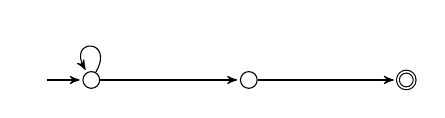
\begin{tikzpicture}[node distance=2cm,bend angle=30]   
	    \node[initial,state] (1) {};  
	    \node[state] (2) [right of=1] {};
	    \node[state,accepting] (3) [right of=2] {};
	    \path[->]
	      (1)   edge  node {} (2)
	      (2)   edge  node {} (3)
	      (1)   edge [swap,in=120,out=60,loop] node {} ();	            
      \end{tikzpicture}     
    }   
    \caption{The automaton .}
    \label{fig ex aut klna}
  \end{figure}
  \end{example}



  The computation of the pairs  for any pair  of a state and a word is sufficient to compute a quasi-deterministic structure. 
  \modif{}{Indeed, for any state , reading  symbols  is enough to compute without ambiguity the unique successor . Hence defining the states of the QDS as couples (state,word) is sufficient.}
  The quasi-deterministic structure is exponentially bigger with respect to the size of the alphabet than the automaton. That has to be compared with the exponential growth with respect to the number of states in the classical determinization.

\begin{definition}\label{def qds}
  Let  be a -unambiguous automaton. The \emph{quasi-deterministic structure associated with}  is    where:
  \begin{itemize}
  \item 
    \item , ,
    \item ,
    \item ,
    \item 




    \item , .
  \end{itemize}
\end{definition}

\modif{}{Let us show that the QDS associated with any -automaton  is exponential w.r.t. the size of the alphabet and recognizes . First, as a direct consequence of Definition~\ref{def qds}, the following proposition holds.}

\begin{proposition}\label{prop taille qds associ}
  Let  be a -unambiguous automaton and  be the quasi-deterministic structure associated with . Then the number of states of  is .
\end{proposition}
\modif{\begin{proof}
  Trivially according to Definition~\ref{def qds}.
  
\end{proof}}{}

\begin{proposition}\label{prop langage qds}
  Let  be a -unambiguous automaton and  be the quasi-deterministic structure associated with . Then\modif{:}{ .}

  \centerline{\modif{.}{}}
\end{proposition}
\begin{proof}
  Let ,  and  be the extended transition function of  (See Definition \ref{def ext delta}). Let  be a word in . Let us show by recurrence on the length of  that:


  \centerline{
    \begin{tabular}{cp{3cm}}
      ,    &  \hfill(\textbf{P1})\\
    \end{tabular}
  }
  Suppose that . We have . According to Definition~\ref{def qds}, \textbf{(a)}  and \textbf{(b)}   . (\textbf{P1}) is satisfied.
  
  Let us suppose that  (\textbf{P1}) is satisfied for any word  such that  . Suppose now that . Either \textbf{(Case I)}  if  or \textbf{(Case II)} . \textbf{Case II} implies that  and consequently  is neither in  nor in . Suppose that \textbf{Case I} holds. By the recurrence hypothesis,   . Since , we have     and  which implies . As a consequence   . Finally    and (\textbf{P1}) holds.
  
  As a conclusion, (\textbf{P1}) holds for  and since for all  in ,   , equality of languages holds.
  
\end{proof}



  \begin{example}\label{ex:quasidetstruct}
   Let us consider the automaton  defined in Example~\ref{ex:calculstep}. After removing unreachable states, the quasi-deterministic structure associated with  is given in Figure~\ref{fig qdet asso ex}.
  \end{example}
  
  \begin{figure}[H]
    \centerline{  
      \begin{tikzpicture}[node distance=2cm,bend angle=30]   
	    \node[initial,state,rounded rectangle] (1eps) {}; 
	    \node[state,rounded rectangle,node distance=7cm,right of=1eps] (1eps2) {};   
	    \node[node distance=4cm,state,rounded rectangle,above right of=1eps] (1a) {};  
	    \node[node distance=4cm,state,rounded rectangle,below right of=1eps] (1b) {};  
	    \node[state,rounded rectangle,above right of=1a,accepting] (1aa) {};   
	    \node[state,rounded rectangle,below right of=1a,accepting] (1ab) {};
	    \node[node distance=1.5cm,state,rounded rectangle,above right of=1aa,accepting] (1aaa) {};   
	    \node[node distance=1.5cm,state,rounded rectangle,below right of=1aa,accepting] (1aab) {};
	    \node[node distance=1.5cm,state,rounded rectangle,above right of=1ab] (1aba) {};   
	    \node[node distance=1.5cm,state,rounded rectangle,below right of=1ab] (1abb) {};
	    \node[state,rounded rectangle,above right of=1b] (1ba) {};   
	    \node[state,rounded rectangle,below right of=1b] (1bb) {};	    \node[node distance=1.5cm,state,rounded rectangle,above right of=1ba,accepting] (1baa) {};   
	    \node[node distance=1.5cm,state,rounded rectangle,below right of=1ba,accepting] (1bab) {};
	    \node[node distance=1.5cm,state,rounded rectangle,above right of=1bb] (1bba) {};   
	    \node[node distance=1.5cm,state,rounded rectangle,below right of=1bb] (1bbb) {}; 
	    \path[->]
	      (1eps)   edge  node {} (1a)
	      (1eps)   edge  node {} (1b)
	      (1a)   edge  node {} (1aa)
	      (1a)   edge  node {} (1ab)
	      (1b)   edge  node {} (1ba)
	      (1b)   edge  node {} (1bb)
	      (1aa)   edge  node {} (1aaa)
	      (1aa)   edge  node {} (1aab)
	      (1ab)   edge  node {} (1aba)
	      (1ab)   edge  node {} (1abb)
	      (1ba)   edge  node {} (1baa)
	      (1ba)   edge  node {} (1bab)
	      (1bb)   edge  node {} (1bba)
	      (1bb)   edge  node {} (1bbb)
	      (1aaa)   edge[dotted,bend right,swap]  node {} (1eps)
	      (1aab)   edge[dotted,bend left]  node {} (1eps2)
	      (1baa)   edge[dotted]  node {} (1eps)
	      (1bab)   edge[dotted]  node {} (1eps2)
	      (1aba)   edge[dotted]  node {} (1eps2)
	      (1bba)   edge[dotted,bend right]  node {} (1eps2)
	      (1abb)   edge[dotted,swap]  node {} (1eps)
	      (1bbb)   edge[dotted,bend left]  node {} (1eps)
	      ;	            
      \end{tikzpicture}     
    }   
    \caption{The Quasi-Deterministic Structure Associated with .}
    \label{fig qdet asso ex}
  \end{figure}
  





\section{Reduction of a quasi-deterministic structure}\label{sec qds}
\modif{}{In this section, we show how to reduce the number of states in a QDS, first by getting rid of  useless states, then by merging equivalent states.}
\subsection{Accessibility and co-accessibility of a QDS}
The definition of trim quasi-deterministic structure differs from the one of trim automaton. Indeed, accessibility and
co-accessibility as defined in automata are not enough 
to obtain
a trim quasi-deterministic structure (see Example~\ref{ex useful} for an illustration). 

\begin{definition}
\modif{}{A state of a QDS is useful if it is on a successful path or if it is initial. A transition is useful if it appears on a successful path. The finality of a state is useful if this state is the destination of a successful path. A QDS is trim if \textbf{(1)}  each state is useful, \textbf{(2)} each transition is useful and \textbf{(3)} the finality of each final state is useful.} 
\end{definition}

\begin{example}\label{ex useful}
  Consider the QDS \modif{}{} in Figure~\ref{fig ex qds trim}. The only useful states are states  and . Indeed, states  and  in Figure~\ref{fig ex qds trim} are not on any shiftable path: using the -transition of label , there is  a symbol  or  in the reading window when the QDS reaches the state . Hence there is no word  such that . Furthermore, since there is no word  such that , and as  is not a final state, both  and  are not useful.
\modif{}{Indeed, ,  and for any integer , .}
\end{example}  

\begin{minipage}[b]{0.49\linewidth}
\begin{figure}[H]
  \centerline{
    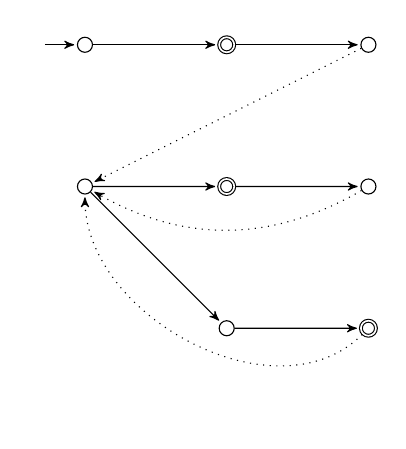
\begin{tikzpicture}[node distance=2cm,bend angle=30,transform shape,scale=0.9]   
	    \node[initial, state] (1) {};     
	    \node[accepting, state, right of=1] (2) {}; 
	    \node[state, right of=2] (4) {}; 
	    \node[state, below of=1] (6) {};  
	    \node[accepting, state, right of=6] (7) {}; 
	    \node[state, right of=7] (8) {};  
	    \node[state, below of=7] (9) {};  
	    \node[state, right of=9,accepting] (10) {};  
	    \path[->]
	      (1)   edge  node {} (2)
	      (2)   edge  node {} (4)
	      (6)   edge  node {} (7)
	      (6)   edge  node {} (9)
	      (7)   edge  node {} (8)
	      (9)   edge  node {} (10)
	      (4)   edge[dotted]  node {} (6)
	      (8)   edge[dotted,bend left]  node {} (6)
	      (10)   edge[in=-90,out=-135,dotted,looseness=1]  node {} (6)
	      ;	            
      \end{tikzpicture}}
  \caption{A Not-trim Quasi-Deterministic Structure.}
  \label{fig ex qds trim}
\end{figure} 
 \end{minipage}  
\begin{minipage}[b]{0.49\linewidth}
\begin{figure}[H]
  \centerline{
    \begin{tikzpicture}[node distance=2cm,bend angle=30,transform shape,scale=0.9]   
	    \node[initial, state] (1) {};     
	    \node[accepting, state, right of=1] (2) {}; 
	     \node[below of=1] (6){};
	    \path[->]
	      (1)   edge  node {} (2);
      \end{tikzpicture}}
  \caption{Its trim part}
\end{figure} 
 \end{minipage}  
\bigskip

\modif{A state is useful if it appears on a successful path or if it is initial. A transition is useful if it appears on a successful path. The finality of a state is useful if this state is the destination of a successful path.
 A trim part of a quasi-deterministic structure can be computed by keeping only useful components. }{ Let us show that the trim part of a QDS is computable.}
Let  be two words of . We denote by  (resp )  if  is a prefix of  ( is a proper prefix of ). 

In order to compute the trim part of a QDS, we need to decide whether a state, an edge or a final state appears on a successful path.  The successful  paths can be computed through the path-DFA associated with any QDS, defined as follows.


\begin{definition}
  Let  be a QDS. The path-DFA of  is the DFA   defined as follows:
  \begin{itemize}
    \item  
    \item 
    \item 
    \item 
    \item 
  \end{itemize}
\end{definition}

\begin{figure}[H]
  \centerline{
    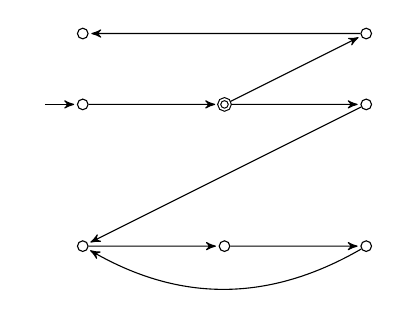
\begin{tikzpicture}[node distance=2cm,bend angle=30,transform shape,scale=0.9]   
	    \node[initial, state, rounded rectangle] (1) {};   
	    \node[ state, rounded rectangle, above of =1,node distance=1cm] (6b) {};     
	    \node[accepting, state, right of=1, rounded rectangle] (2) {}; 
	    \node[state, right of=2, rounded rectangle] (4) {}; 
	    \node[state, above of=4, rounded rectangle, node distance=1cm] (4b) {}; 
	    \node[state, below of=1, rounded rectangle] (6) {};  
	    \node[ state, right of=6, rounded rectangle] (7) {}; 
	    \node[state, right of=7, rounded rectangle] (8) {}; 
	    \path[->]
	      (1)   edge  node {} (2)
	      (2)   edge  node {} (4)
	      (2)   edge  node {} (4b)
	      (6)   edge  node {} (7)
	      (7)   edge  node {} (8)
	      (4)   edge  node {} (6)
	      (4b)   edge  node {} (6b)
	      (8)   edge[bend left]  node {} (6)
	      ;	            
      \end{tikzpicture}  
  }
  \caption{The  Path-DFA of the QDS of Figure \ref{fig ex qds trim}.}
\end{figure}  

  
  \modif{}{Let us now explicit the relation between the shiftable paths of a QDS and a path in the associated path-DFAs.}

\begin{theorem}\label{link-QDS-pathDFA}
  Let   be a QDS. Let   be the path-DFA of . The three following conditions hold:
  \begin{enumerate}
    \item A state  is useful  if and only if there exists a useful state  in .
    \item A transition  is useful if and only if there exists a transition  in  where the states  and  are useful.\item The finality of the state  is useful if and only if there exists a final useful state  in .
  \end{enumerate}
\end{theorem}

The notion of successful path in a QDS can be expressed through the notion of successful path in its associated path-DFA.

\begin{lemma}\label{lem-shift}
 Let  be a QDS and  be its path-DFA. Let  be a word over  and  be a path in . The two following conditions are equivalent:
  \begin{enumerate}
    \item The path  is shiftable,
    \item  there exists two words  with  and a path  in  labelled  from  to .
  \end{enumerate}
  Moreover,  is successful in  if and only if  is successful in .
\end{lemma}
\begin{proof}
\ \\
\begin{itemize}
\item[] By recurrence on the number  of -transitions in . If , then  is in . By construction, there exists a path  in  labelled  from  to . Let us show the property for a path with  -transitions. Then   with  the  -transition of . By definition of a shiftable path,  is shiftable and then by the recurrence hypothesis there exists a path in  from  to  with .
By construction of , . As  is shiftable, we have . So, by construction, there exists a path in  from  to  with  in  and  which ends the proof.
\item[] By recurrence on the number  of transitions labelled by a symbol of  in  (-transitions). If  then . Consequently, the path  of  is shiftable. Let us show the property for a path with  -transitions. Let    with   the last -transition of . By the induction hypothesis   implies that the path  is a shiftable path in . As there exists a path from  to  in  with , . So  and so  is a shiftable path.
\end{itemize}
\end{proof}
\begin{proof}(of Theorem \ref{link-QDS-pathDFA})
Conditions ,  and  directly holds  from Definition \ref{def successful} and Lemma \ref{lem-shift}.
\end{proof}








\begin{example}\label{ex path DFA}
  Consider the QDS in Figure~\ref{fig ex qds path dfa} \modif{}{(the  QDS of  Figure~\ref{fig ex qds trim} in which the state  has been made final)}.  The states  and  are not accessible, the transition  is not useful, and neither is the finality of . The accessible part of its path-DFA is given Figure~\ref{fig ex dfa path dfa} and its trim part in Figure~\ref{fig ex trim qds path dfa}.
\end{example}  

\begin{minipage}[b]{0.49\linewidth}
\begin{figure}[H]
  \centerline{
    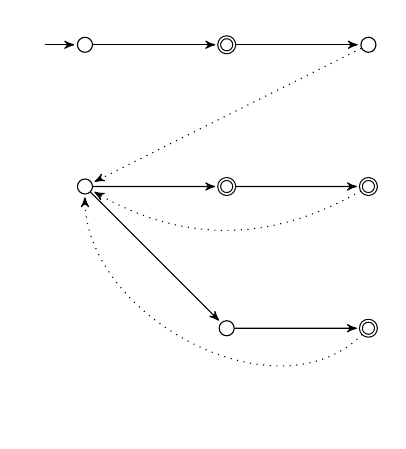
\begin{tikzpicture}[node distance=2cm,bend angle=30,transform shape,scale=0.9]   
	    \node[initial, state] (1) {};     
	    \node[accepting, state, right of=1] (2) {}; 
	    \node[state, right of=2] (4) {}; 
	    \node[state, below of=1] (6) {};  
	    \node[accepting, state, right of=6] (7) {}; 
	    \node[accepting,state, right of=7] (8) {};  
	    \node[state, below of=7] (9) {};  
	    \node[state, right of=9,accepting] (10) {};  
	    \path[->]
	      (1)   edge  node {} (2)
	      (2)   edge  node {} (4)
	      (6)   edge  node {} (7)
	      (6)   edge  node {} (9)
	      (7)   edge  node {} (8)
	      (9)   edge  node {} (10)
	      (4)   edge[dotted]  node {} (6)
	      (8)   edge[dotted,bend left]  node {} (6)
	      (10)   edge[in=-90,out=-135,dotted,looseness=1]  node {} (6)
	      ;	            
      \end{tikzpicture}  
  }
  \caption{A Quasi-Deterministic Structure .}\label{fig ex qds path dfa}
\end{figure} 
\end{minipage}
\begin{minipage}[b]{0.49\linewidth}
\begin{figure}[H]
  \centerline{
    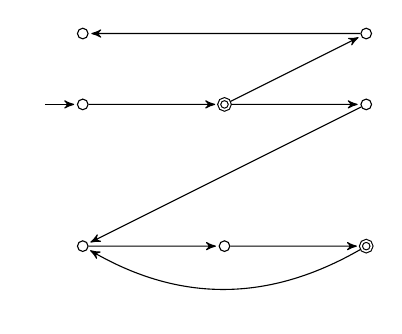
\begin{tikzpicture}[node distance=2cm,bend angle=30,transform shape,scale=0.9]   
	    \node[initial, state, rounded rectangle] (1) {};   
	    \node[ state, rounded rectangle, above of =1,node distance=1cm] (6b) {};     
	    \node[accepting, state, right of=1, rounded rectangle] (2) {}; 
	    \node[state, right of=2, rounded rectangle] (4) {}; 
	    \node[state, above of=4, rounded rectangle, node distance=1cm] (4b) {}; 
	    \node[state, below of=1, rounded rectangle] (6) {};  
	    \node[ state, right of=6, rounded rectangle] (7) {}; 
	    \node[accepting,state, right of=7, rounded rectangle] (8) {}; 
	    \path[->]
	      (1)   edge  node {} (2)
	      (2)   edge  node {} (4)
	      (2)   edge  node {} (4b)
	      (6)   edge  node {} (7)
	      (7)   edge  node {} (8)
	      (4)   edge  node {} (6)
	      (4b)   edge  node {} (6b)
	      (8)   edge[bend left]  node {} (6)
	      ;	            
      \end{tikzpicture}  
  }
\caption{The Path-DFA of S.}
  \label{fig ex dfa path dfa}
\end{figure}  
\end{minipage}

\begin{minipage}[b]{0.49\linewidth}
\begin{figure}[H]
  \centerline{
    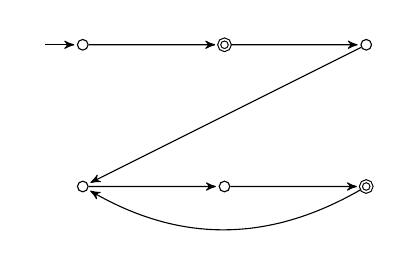
\begin{tikzpicture}[node distance=2cm,bend angle=30,transform shape,scale=0.9]   
	    \node[initial, state, rounded rectangle] (1) {};   
\node[accepting, state, right of=1, rounded rectangle] (2) {}; 
	    \node[state, right of=2, rounded rectangle] (4) {}; 
\node[state, below of=1, rounded rectangle] (6) {};  
	    \node[ state, right of=6, rounded rectangle] (7) {}; 
	    \node[accepting,state, right of=7, rounded rectangle] (8) {}; 
	    \path[->]
	      (1)   edge  node {} (2)
	      (2)   edge  node {} (4)
(6)   edge  node {} (7)
	      (7)   edge  node {} (8)
	      (4)   edge  node {} (6)
(8)   edge[bend left]  node {} (6)
	      ;	            
      \end{tikzpicture}  
  }
  \caption{The Trim  Path-DFA.}
\label{fig trim ex dfa path dfa}
\end{figure}  
\end{minipage}
\begin{minipage}[b]{0.49\linewidth}
\begin{figure}[H]
  \centerline{
    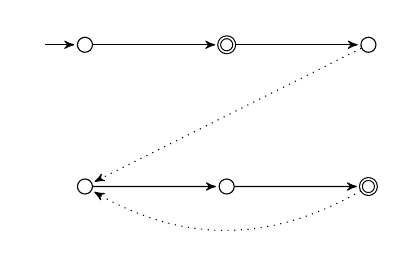
\begin{tikzpicture}[node distance=2cm,bend angle=30,transform shape,scale=0.9]   
\node[initial, state] (1) {};     
	    \node[accepting, state, right of=1] (2) {}; 
	    \node[state, right of=2] (4) {}; 
	    \node[state, below of=1] (6) {};  
	    \node[state, right of=6] (7) {}; 
	    \node[accepting,state, right of=7] (8) {};  
	    \path[->]
	      (1)   edge  node {} (2)
	      (2)   edge  node {} (4)
	      (6)   edge  node {} (7)
	      (7)   edge  node {} (8)
	      (4)   edge[dotted]  node {} (6)
	      (8)   edge[dotted,bend left]  node {} (6)
	      ;	            
      \end{tikzpicture}  
  }
  \caption{The Trim version of .}\label{fig ex trim qds path dfa}
\end{figure} 
\end{minipage}




\modif{}{As a direct consequence of Corollary~\ref{Cor-1}, we have:}

 \begin{lemma}
 Let  be the trim part of a QDS . Then .
 \end{lemma}
 \modif{\begin{proof}
 The proof is a direct consequence of Corollary~\ref{Cor-1}
 \end{proof}}{}








 In the following, we will consider trim QDS.

\subsection{Defining an equivalence relation  for a QDS}

The minimization process in a DFA consists in merging each 
couple of states having the same right language.
The \emph{right language of a state}  is defined as the set of words  such that  is a final state. This computation leads to the canonical minimal DFA.

In a quasi-deterministic structure, the notion of right language can not be defined as in an automaton. Indeed, even if a state is useful, it can be not accessible. Thus, we \modif{can}{must} define an equivalence relation allowing us to reduce the size of a QDS. Notice that this
equivalence is sufficient
to reduce the number of states, but not to minimize: modifying the values of some -transitions might preserve the language while producing equivalent states.

Let  be a QDS. The reduced QDS is always computed from a QDS not recognizing the empty word. Obviously, if  recognizes , necessarily . In this case,  is removed from  to compute the reduced QDS  recognizing . The initial state of  is then made final to have . Indeed, the finality of each final state of  is not useful, excepted for  if .

We define an equivalence relation  over . Let , .


 

 \noindent
We denote .\\
  
  
The \emph{quotient of}  with respect to  is the QDS  defined by:
  \begin{itemize}
    \item , ,
\item , 
\item , , ,
    \item ,  with .
  \end{itemize}  
  \modif{where for any state , .}{}
  
  We first show that merging two equivalent states preserves the language. This property is sufficient, but not necessary. 

\begin{proposition}\label{prop rightinv pres lang}
  Let  be a QDS and    be the quotient of  with respect to . We have:
  
  \centerline{
    .
  }
\end{proposition}
\begin{proof}
Let  be the extended transition function of .
  \begin{enumerate}
    \item Let us consider the empty word :
  
  \centerline{
               \modif{  }{}    
  }
  
  \item Let  be a word in . Let us show by recurrence on the length of  that for any element  in ,   .
  
   \begin{enumerate}
     \item Suppose that . Then:
  
\begin{tabular}{ll@{\ }l}
         &
         &   
          \\
       &   &  .\\
    \end{tabular}


 \item Suppose that . Then: 

    \begin{tabular}{l@{\ }l@{\ }l}
       
      &   & \\
      &  &  \\
      &  &  \\
      & & (According to  \modif{}{the} recurrence hypothesis)\\
      &  & \\
    \end{tabular}
\end{enumerate}
  
  \item Finally, since for any element  in , for any word  in ,   , it holds:
  
  \centerline{
       and .
  }
  \end{enumerate}
  
\end{proof}



\subsection{Computing the equivalence relation }

In this section, we show how to compute step by step the equivalence relation   which merges states of  a QDS.

\begin{definition}\label{def equiv}
  Let  be a QDS. Let , . We define  the equivalence relation  over   by:
  
    
    
  
  


\end{definition}



For the purposes of notation,  designates the set of  class of this equivalence relation. By definition, we have . It is obvious that  is computable from . We give several lemmas to show that this computation halts and is bounded by . 


\begin{lemma}
Let   be a QDS.  For any integer , 
   \end{lemma}
   \begin{proof}
Let  be the integer such that .
Then, there exists ,   such that , , and .
But  implies that there exists  such that condition  is false (impossible for condition ).
In this case,
if , . But by hypothesis , then
 and then  which leads to a contradiction.

If , .
By hypothesis, we have , that is , and
. This would imply . Contradiction.
   \end{proof}


\begin{lemma}
Let   be a QDS.   
   \end{lemma}
   \begin{proof}

 
 The smallest integer  such that  is the highest integer such that . Since the smallest difference between two consecutive equivalences is based on the elimination of only one state, it holds that such an integer  exists and .
  
\end{proof}











\section{QDS can be exponentially smaller than DFAs}\label{sec qds vs dfa}



Let  be the family of regular languages on an alphabet    defined by  with . This family is known to have a -states NFA and a 
-states minimal DFA.
In this section, we illustrate the factorization power of QDS. We show how to compute a polynomial-size QDS   recognizing  (See  Figure~\ref{fig ex qds reck}).



\begin{definition}
  Let  be an integer. We denote by  the quasi-deterministic structure  defined by:
  \begin{itemize}
    \item , \item , , ,
\item ,
    \item ,
    \item 
    \item 
  \end{itemize}
\end{definition}





\begin{example}

The QDS  is represented by Figure \ref{fig ex qds reck} where the arrows of  are respectively coded by 
 for \textbf{(1)},  for \textbf{(2)},  for \textbf{(3)},  for \textbf{(4)},  for \textbf{(5)},  for \textbf{(6)} and  for \textbf{(7)}.
The arrows of  are represented by .
\begin{figure}[H]
\begin{tikzpicture}[node distance=2cm,bend angle=30,transform shape]   
	    \node[initial, state] (11) at (0,0) {};     
	    \node[state] (32) at (2.5,0.7) {};     
              \node[state] (22) at (2.5,2.1) {};     
              \node[state] (12) at (2.5,3.5) {};     
	    \node[state] (12p) at (2.5,-0.7) {};     
              \node[state] (22p) at (2.5,-2.1) {};     
              \node[state] (32p) at (2.5,-3.5) {};     
\node[state] (33) at (5,0.7) {};     
              \node[state] (23) at (5,2.1) {};     
              \node[state] (13) at (5,3.5) {};     
	    \node[state] (13p) at (5,-0.7) {};     
              \node[state] (23p) at (5,-2.1) {};     
              \node[state] (33p) at (5,-3.5) {};     
\node[state,accepting] (34) at (7.5,0.7) {};     
              \node[state,accepting] (24) at (7.5,2.1) {};     
              \node[state,accepting] (14) at (7.5,3.5) {};     
	    \node[state] (14p) at (7.5,-0.7) {};     
              \node[state] (24p) at (7.5,-2.1) {};     
              \node[state] (34p) at (7.5,-3.5) {};     
\node[state,accepting] (15) at (10,2.1) {};     
              \node[state] (25) at (10,0.7) {};     
              \node[state] (35) at (10,-0.7) {};     
              \node[state] (45) at (10,-2.1) {};     
\path[->]
	      (11)   edge[green,loosely dashdotted]  node {} (12)
	                edge[green,loosely dashdotted ] node {} (12p)
	        (12) edge[red,decorate,decoration={snake,amplitude=.4mm,segment length=2mm,post length=1mm},densely dotted]  node {} (13)        
	        (12p) edge[red,decorate,decoration={snake,amplitude=.4mm,segment length=2mm,post length=1mm},densely dotted]  node {} (13p)        
  	        (23) edge[red,decorate,decoration={snake,amplitude=.4mm,segment length=2mm,post length=1mm},densely dotted]  node {} (24)        
	        (23p) edge[red,decorate,decoration={snake,amplitude=.4mm,segment length=2mm,post length=1mm},densely dotted]  node {} (24p)        
	        (13) edge  node {} (14)        
  	        (13p) edge  node {} (14p)       
	        (12) edge[red,decorate,decoration={snake,amplitude=.4mm,segment length=2mm,post length=1mm},densely dashed]  node {} (23)        
	        (23) edge[red,decorate,decoration={snake,amplitude=.4mm,segment length=2mm,post length=1mm},densely dashed]  node {} (34)        
	        (12p) edge[red,decorate,decoration={snake,amplitude=.4mm,segment length=2mm,post length=1mm},densely dashed]  node {} (23p)        
	        (23p) edge[red,decorate,decoration={snake,amplitude=.4mm,segment length=2mm,post length=1mm},densely dashed] node {} (34p)       
	        (14) edge[decorate,decoration={snake,amplitude=.4mm,segment length=2mm,post length=1mm}]  node {} (15)        
	         (24) edge[decorate,decoration={snake,amplitude=.4mm,segment length=2mm,post length=1mm}]   node {} (25)        
	        (34) edge[green,dashed]  node {} (35)        
	         (34) edge[densely dashdotted]  node [swap,pos=0.65]{} (45)        
	        (34p) edge[green, dashed]  node {} (35)        
	         (34p) edge[densely dashdotted]  node[swap] {} (45)    
	         (14p) edge[decorate,decoration={snake,amplitude=.4mm,segment length=2mm,post length=1mm}] node {}(15)	          
	         (24p) edge[decorate,decoration={snake,amplitude=.4mm,segment length=2mm,post length=1mm}] node[pos=0.3] {}(25)	          
(15)   edge[dotted,in=90, out=70,looseness=1.3,swap]  node[swap] {} (11)
	      (25)   edge[dotted,in=90, out=45,looseness=2,swap]  node {} (11)
	      (35)   edge[dotted,in=-90, out=-45,looseness=2]  node {} (11)
	      (45)   edge[in=-90, out=-70,dotted,looseness=1.3]  node[swap] {} (11);
\end{tikzpicture}  
\caption{The QDS .}
	  \label{fig ex qds reck}
	\end{figure} 
\end{example}

\begin{proposition}\label{prop Sk bon lang}
   For any integer , the QDS  recognizes .
\end{proposition}
\begin{proof}
  Let  be a word in . Let us denote . We show by recurrence on  that    .
  
\textbf{(I)} 
  \begin{itemize} 
  \item Let . By definition,  has  levels. Final states of  are on levels  and . Thus,  is not recognized by . As , the minimal length of any recognized word is . Thus, when , . 
 \item Let . If , necessarily . By construction, . Thus . Conversely, if , . Necessarily,  and then . 
\item Let .  If , necessarily . By ,   and by , as ,  and . Moreover, by ,  and  for . To conclude, by ,  and , so . Conversely, if , . By  there exists  such that . By , there exists  such that  which implies . As  is directly accessible from the initial state, .
  \end{itemize}
  \textbf{(II)} Let us suppose that . We show by recurrence on  that: 
  \begin{itemize}
    \item   \hfill (a)
    \item   \hfill (b)
    \item , , 
      \begin{itemize}
        \item    \hfill (c)
        \item   \hfill (d)
        \item   \hfill (e)
        \item   \hfill (f)
      \end{itemize}
    \item ,   \hfill (g)  
    \item   \hfill (h)
  \end{itemize}
  


Let us suppose that the recurrence  holds for any integer . Let  with  in  and . Let us suppose that:
  
  \begin{itemize}
    \item[\textbf{(a)}] .  Then  . By definition, .
    If ,  and  (case (c) with  and ).
    If ,  and  (case (d) with ).
\item[\textbf{(b)}] . By \modif{}{the} recurrence hypothesis, . If ,  and  (case (e) with  and ).
    If ,  and  (case (f) with ).
\item[\textbf{(c)}]  with  and . If , then by \modif{}{the} recurrence hypothesis, .  By definition of  (4),   and . 
    By substituting ,  and  (case (c)).
If , then by \modif{}{the} recurrence hypothesis, . Hence  and  (case (g)).
\item[\textbf{(d)}]  with .  Then by \modif{}{the} recurrence hypothesis, . If ,  and . By substituting  and ,  and  (case (c)).
    If ,  and . Then,  and  (case (d)).   \item[\textbf{(e)}]   with  and .  If , then by \modif{}{the} recurrence hypothesis, . 
By definition of ,  and . By substituting ,  and  (case (e)).
If , then by \modif{}{the} recurrence hypothesis, . Hence  and  (case (g)).
\item[\textbf{(f)}]   with .  Then by \modif{}{the} recurrence hypothesis, . If ,  and . By substituting  and ,  and  (case (e)).
If ,  and  (case (f)).
\item[\textbf{(g)}]   with . 
    Then by \modif{}{the} recurrence hypothesis, . 
    Consequently, ,  and .
    By definition of , .
Furthermore, .
    Hence . So  and the cases (c), (d) and (g) have to be considered.
Hence \modif{}{the} recurrence holds. 


    \item[\textbf{(h)}] .  Then by \modif{}{the} recurrence hypothesis, . 
    If ,  and  (case (a)). 
    If ,  and  (case (b)). 
    Hence \modif{}{the} recurrence holds. 
  \end{itemize}
  


  \textbf{(III)} Finally, since , and since for any ,  is defined, it holds that   .
  
\end{proof}

\modif{}{As a direct consequence of Proposition~\ref{prop Sk bon lang}, it holds:}
\begin{theorem}\label{thm qds expo smaller}
  There exists a QDS  that recognizes  which is exponentially smaller than the minimal DFA associated with .
\end{theorem}
\modif{\begin{proof}
  Corollary of Proposition~\ref{prop Sk bon lang}.
  
\end{proof}}{}





 








\section{Conclusion and Perspectives}

Quasi-deterministic structures are an alternative to the computation of a deterministic automaton since they can be used as recognizers, while reducing the space needed to solve the membership problem once computed.
We have  shown that reduced QDSs can be exponentially smaller than equivalent deterministic automata. 








A regular language is -unambiguous if it is denoted by some regular expression the position automaton of which is -unambiguous. 
Similar extensions were already defined for deterministic automata (-unambiguity). 
Denoting a language by such an expression allows us to directly compute a quasi-deterministic structure in order to solve the membership problem.  
  
One may wonder whether every regular language admits a -unam\-biguous position automaton recognizing it.
If the answer is negative, then a second question arises: Is it possible to characterize languages having a -unam\-biguous position automaton, as Br\"uggemann-Klein and Wood did for languages having a deterministic position automaton ?





\section*{References}
\bibliography{/Users/pacot/TEX/BIBLIO/biblio}







  



\end{document}
